\documentclass{standalone}

\usepackage{tikz}
\usepackage{ctex}

\begin{document}
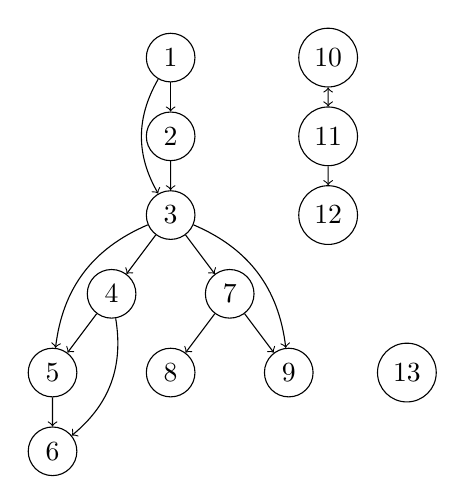
\begin{tikzpicture}
    [level distance=10mm,every node/.style={draw,circle}]

\node (A) at (0,0) {$1$}
    child[->] {node (B) {$2$}
        child {node (C) {$3$}
            child {node (D) {$4$}
                child {node (E) {$5$}
                    child {node (F) {$6$}}
                }
                child[missing]
            }
            child {node (G) {$7$}
                child {node (H) {$8$}}
                child {node (I) {$9$}}
            }
        }
    };

\node (J) at (2,0) {$10$}
    child[<->] {node (K) {$11$}
        child[->] {node (L) {$12$}}};

\node (M) at (3,-4) {$13$};

\path[->]
    (A) edge[bend right] (C)
    (C) edge[bend right] (E)
    (D) edge[bend left] (F)
    (C) edge[bend left] (I);

\end{tikzpicture}
\end{document}
